\documentclass[12pt,a4paper]{article}

% --- Page Layout -------------------------------------------------------------
\usepackage[a4paper, margin=0.8in, headheight=14pt]{geometry}

% --- Fonts (XeLaTeX) ---------------------------------------------------------
\usepackage{fontspec}
\usepackage{unicode-math}
\setmainfont{TeX Gyre Pagella}
\setmonofont[Scale=0.88]{TeX Gyre Cursor}
\setmathfont{Latin Modern Math}

% --- Packages ---------------------------------------------------------------
\usepackage{xcolor}
\usepackage{titlesec}
\usepackage{enumitem}
\usepackage{tabularx}
\usepackage{booktabs}
\usepackage{array}
\usepackage{amsmath}
\usepackage{tikz}
\usetikzlibrary{shapes.geometric, arrows.meta, positioning, calc, fit, decorations.pathreplacing}
\usepackage{tcolorbox}
\tcbuselibrary{skins, breakable}
\usepackage{hyperref}
\usepackage{fancyhdr}
\usepackage{graphicx}
\usepackage{microtype}
\hyphenpenalty=10000
\exhyphenpenalty=10000
\sloppy
\usepackage{caption}
\usepackage{setspace}
\usepackage{multirow}
\usepackage{tocloft}

% --- Q&A helper --------------------------------------------------------------
\newcommand{\Q}[1]{\textbf{#1}\par\noindent\ignorespaces}

% --- Colour Palette ----------------------------------------------------------
\definecolor{myred}{RGB}{196,30,58}
\definecolor{mydark}{RGB}{30,30,50}
\definecolor{mygreen}{RGB}{14,120,80}
\definecolor{myteal}{RGB}{0,130,140}
\definecolor{myamber}{RGB}{180,100,0}
\definecolor{mypurple}{RGB}{100,30,160}
\definecolor{mygray}{RGB}{246,247,249}
\definecolor{mgframe}{RGB}{180,185,200}
\definecolor{watermark}{RGB}{145,150,170}
\definecolor{hdrred}{RGB}{250,232,235}
\definecolor{hdrgreen}{RGB}{220,244,233}
\definecolor{hdrteal}{RGB}{220,242,244}
\definecolor{hdramber}{RGB}{253,242,215}
\definecolor{hdrpurple}{RGB}{238,228,255}
\definecolor{hdrgray}{RGB}{238,240,245}
\definecolor{rowalt}{RGB}{250,251,253}

% --- Section Formatting ------------------------------------------------------
\titleformat{\section}
  {\large\bfseries\color{myred}}{\thesection.}{0.5em}{}
  [\vspace{1pt}{\color{myred}\rule{\linewidth}{0.8pt}}]
\titleformat{\subsection}
  {\normalsize\bfseries\color{myteal}}{\thesubsection}{0.5em}{}
\titlespacing*{\section}{0pt}{18pt}{7pt}
\titlespacing*{\subsection}{0pt}{11pt}{4pt}

% --- Paragraph ---------------------------------------------------------------
\setlength{\parindent}{0pt}
\setlength{\parskip}{4pt}

% --- TOC Styling -------------------------------------------------------------
\renewcommand{\cfttoctitlefont}{\large\bfseries\color{myred}}
\renewcommand{\cftaftertoctitle}{\par\noindent{\color{myred}\rule{\linewidth}{0.8pt}}}
\setlength{\cftbeforetoctitleskip}{0pt}
\setlength{\cftaftertoctitleskip}{6pt}
\renewcommand{\cftsecfont}{\normalsize\bfseries\color{mydark}}
\renewcommand{\cftsecpagefont}{\normalsize\bfseries\color{mydark}}
\renewcommand{\cftsecleader}{\cftdotfill{\cftdotsep}}
\setlength{\cftbeforesecskip}{7pt}
\renewcommand{\cftsubsecfont}{\small\color{mydark}}
\renewcommand{\cftsubsecpagefont}{\small\color{mydark}}
\setlength{\cftbeforesubsecskip}{3pt}
\setlength{\cftsubsecindent}{1.4em}

% --- Table helpers -----------------------------------------------------------
\renewcommand{\arraystretch}{1.45}
\setlength{\tabcolsep}{6pt}
\newcolumntype{B}[1]{>{\small\bfseries\raggedright\arraybackslash}m{#1}}
\newcolumntype{Y}{>{\small\raggedright\arraybackslash}X}
\renewcommand{\tabularxcolumn}[1]{m{#1}}

% --- Header / Footer ---------------------------------------------------------
\pagestyle{fancy}
\fancyhf{}
\fancyhead[L]{\small\color{myred}\textbf{BS-CH101}\;\color{mydark}--- Chemistry-I}
\fancyhead[R]{\small\color{myteal}\textbf{Module 2 Notes}}
\fancyfoot[C]{\small\color{mydark}\thepage}
\fancyfoot[R]{\small\color{watermark}\textit{\copyright\ Biraj}}
\renewcommand{\headrulewidth}{0.5pt}
\renewcommand{\footrulewidth}{0.3pt}

% --- Hyperref ---------------------------------------------------------------
\hypersetup{
  colorlinks=true, linkcolor=myteal, urlcolor=myteal,
  pdfauthor={Biraj Sarkar},
  pdftitle={BS-CH101 --- Module 2 Notes}
}

% --- tcolorbox styles --------------------------------------------------------
\tcbset{
  tikzbox/.style={
    colback=mygray, colframe=mgframe, boxrule=0.6pt, arc=4pt,
    left=8pt, right=8pt, top=6pt, bottom=6pt,
    colbacktitle=mgframe, coltitle=mydark,
    fonttitle=\small\bfseries
  },
  defbox/.style={
    colback=hdrgreen, colframe=mygreen, boxrule=0.8pt, arc=4pt,
    left=9pt, right=9pt, top=6pt, bottom=6pt,
    colbacktitle=mygreen, coltitle=white,
    fonttitle=\small\bfseries
  },
  formulabox/.style={
    colback=hdrteal, colframe=myteal, boxrule=0.8pt, arc=4pt,
    left=9pt, right=9pt, top=7pt, bottom=7pt,
    colbacktitle=myteal, coltitle=white,
    fonttitle=\small\bfseries
  },
  examplebox/.style={
    colback=hdramber, colframe=myamber, boxrule=0.8pt, arc=4pt,
    left=9pt, right=9pt, top=6pt, bottom=6pt,
    colbacktitle=myamber, coltitle=white,
    fonttitle=\small\bfseries
  },
  masonbox/.style={
    colback=hdrpurple, colframe=mypurple, boxrule=0.8pt, arc=4pt,
    left=9pt, right=9pt, top=6pt, bottom=6pt,
    colbacktitle=mypurple, coltitle=white,
    fonttitle=\small\bfseries
  },
  exambox/.style={
    colback=hdrpurple, colframe=mypurple, boxrule=1pt, arc=5pt,
    left=10pt, right=10pt, top=8pt, bottom=8pt,
    colbacktitle=mypurple, coltitle=white,
    fonttitle=\bfseries,
    breakable, title after break={\textbf{Frequently Asked / Viva Questions (contd.)}}}
}
\tcbset{breakable}

% --- TikZ styles -------------------------------------------------------------
\tikzset{
  block/.style={rectangle, draw=myteal, fill=hdrteal,
    text width=2.4cm, align=center, minimum height=0.95cm,
    font=\small, rounded corners=3pt, line width=0.7pt},
  redblock/.style={rectangle, draw=myred, fill=hdrred,
    text width=2.4cm, align=center, minimum height=0.95cm,
    font=\small, rounded corners=3pt, line width=0.7pt},
  netnode/.style={rectangle, draw=myteal, fill=hdrteal,
    text width=1.5cm, align=center, minimum height=0.8cm,
    font=\small, rounded corners=3pt, line width=0.7pt},
  sumjunc/.style={circle, draw=myamber, fill=hdramber,
    minimum size=0.62cm, font=\small, line width=0.8pt},
  snode/.style={circle, draw=mypurple, fill=hdrpurple,
    minimum size=0.55cm, font=\footnotesize, line width=0.7pt},
  arrow/.style={-Stealth, thick, color=mydark},
  redarrow/.style={-Stealth, thick, color=myred},
  line/.style={thick, color=mydark}
}

\begin{document}

\begin{center}
  {\LARGE\bfseries\color{myred} BS-CH101 / BS-CH201 --- Chemistry-I}\\[5pt]
  {\normalsize\color{mydark} Semester I \quad$\bullet$\quad 3L:1T:0P \quad$\bullet$\quad 4 Credits}\\[3pt]
  {\normalsize\color{myteal}\textbf{Module 2 Exam Notes: Spectroscopic Techniques and Applications}}\\[3pt]
  {\small\color{mydark} CGEC \;$|$\; B.Tech ECE (2023--27) \;$|$\; \textit{Biraj Sarkar}}
\end{center}
\vspace{2pt}
\noindent{\color{myred}\rule{\linewidth}{1.5pt}}
\vspace{2pt}

\hypersetup{linkcolor=mydark}
\tableofcontents
\hypersetup{linkcolor=myteal}
\newpage
% ===============================================================================
\section{Spectroscopic Techniques and Applications}
% ===============================================================================

\begin{tcolorbox}[defbox]
\textbf{Spectroscopy} is the study of interaction between electromagnetic radiation and matter. It is used to identify molecules, determine structure, and study energy-level transitions.
\end{tcolorbox}

\subsection{Basic Principle and Selection Rules}
When radiation of frequency $\nu$ is absorbed or emitted, a molecule moves between two energy levels.

\begin{tcolorbox}[formulabox, title={Energy of Radiation}]
\[
\Delta E=h\nu=\frac{hc}{\lambda}
\]
where $h$ is Planck's constant, $\nu$ is frequency, $c$ is speed of light, and $\lambda$ is wavelength.
\end{tcolorbox}

A transition is allowed only when it satisfies the required selection rule and has a changing electric or magnetic moment.

\begin{tabularx}{\linewidth}{|B{3cm}|Y|Y|}
\hline
\textbf{Technique} & \textbf{Energy change} & \textbf{Common selection rule} \\
\hline
Rotational & Molecular rotation & $\Delta J=\pm 1$ \\
\hline
Vibrational & Bond vibration & $\Delta v=\pm 1$ for fundamental transition \\
\hline
Electronic & Electron promotion & Spin and symmetry allowed transitions are intense \\
\hline
NMR & Nuclear spin orientation & Nuclei must have non-zero spin \\
\hline
\end{tabularx}

\subsection{Electronic Spectroscopy}
Electronic spectroscopy uses UV-visible radiation. It involves transitions such as $\sigma\rightarrow\sigma^*$, $n\rightarrow\sigma^*$, $\pi\rightarrow\pi^*$, and $n\rightarrow\pi^*$.

\begin{tcolorbox}[tikzbox, title={Common Electronic Transitions}]
\centering
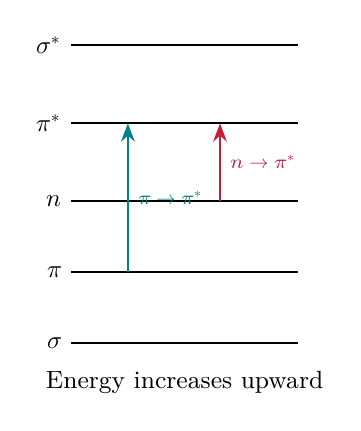
\begin{tikzpicture}[scale=0.9]
  \foreach \y/\lab in {0/$\sigma$,1.0/$\pi$,2.0/$n$,3.1/$\pi^*$,4.2/$\sigma^*$} {
    \draw[thick] (0,\y) -- (3.2,\y);
    \node[left,font=\small] at (0,\y) {\lab};
  }
  \draw[arrow,myteal] (0.8,1.0) -- (0.8,3.1) node[midway,right,font=\scriptsize] {$\pi\rightarrow\pi^*$};
  \draw[arrow,myred] (2.1,2.0) -- (2.1,3.1) node[midway,right,font=\scriptsize] {$n\rightarrow\pi^*$};
  \node[font=\small] at (1.6,-0.55) {Energy increases upward};
\end{tikzpicture}
\end{tcolorbox}

\subsection{Fluorescence and Medical Applications}
Fluorescence occurs when a molecule absorbs light and quickly emits lower-energy light. It is useful in diagnostics, bio-imaging, and detection of trace biomolecules.

\begin{tcolorbox}[tikzbox, title={Jablonski Diagram for Fluorescence}]
\centering
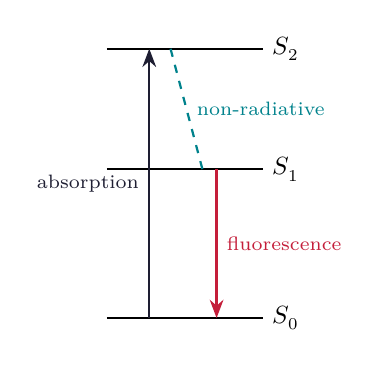
\begin{tikzpicture}[scale=0.9]
  \draw[thick] (0,0) -- (2.2,0) node[right,font=\small] {$S_0$};
  \draw[thick] (0,2.1) -- (2.2,2.1) node[right,font=\small] {$S_1$};
  \draw[thick] (0,3.8) -- (2.2,3.8) node[right,font=\small] {$S_2$};
  \draw[arrow] (0.6,0) -- (0.6,3.8) node[midway,left,font=\scriptsize] {absorption};
  \draw[redarrow] (1.55,2.1) -- (1.55,0) node[midway,right,font=\scriptsize] {fluorescence};
  \draw[thick, dashed, myteal] (0.9,3.8) -- (1.35,2.1) node[midway,right,font=\scriptsize] {non-radiative};
\end{tikzpicture}
\end{tcolorbox}

\subsection{Vibrational and Rotational Spectroscopy}
IR spectroscopy studies molecular vibrations. A vibration is IR active if it changes dipole moment. Rotational spectroscopy is observed mainly for gas-phase polar molecules.

\begin{tcolorbox}[formulabox, title={Vibrational Frequency of a Diatomic Molecule}]
\[
\nu=\frac{1}{2\pi}\sqrt{\frac{k}{\mu}},\qquad
\mu=\frac{m_1m_2}{m_1+m_2}
\]
where $k$ is force constant and $\mu$ is reduced mass.
\end{tcolorbox}

\subsection{NMR, MRI, Surface Characterisation, Diffraction}
NMR detects nuclei in a magnetic field. MRI is a medical imaging application of NMR, mainly using hydrogen nuclei in water and fat. Surface characterisation methods such as XPS, SEM, and AFM help study surface composition and morphology. Diffraction and scattering reveal crystal structure, particle size, and defects.

\begin{tcolorbox}[formulabox, title={Bragg Equation}]
\[
n\lambda=2d\sin\theta
\]
Here $d$ is interplanar spacing and $\theta$ is the Bragg angle.
\end{tcolorbox}

\begin{tcolorbox}[exambox, title={Exam Points}]
\begin{itemize}[leftmargin=*, itemsep=2pt, topsep=2pt]
  \item Mention the energy region: microwave for rotational, IR for vibrational, UV-visible for electronic.
  \item In fluorescence answers, draw the Jablonski diagram.
  \item For NMR/MRI, write the need for non-zero nuclear spin.
  \item For X-ray diffraction, Bragg equation is compulsory.
\end{itemize}
\end{tcolorbox}

% ===============================================================================
\section{Detailed Spectroscopy Notes for Exam Answers}
% ===============================================================================

\subsection{Electromagnetic Spectrum and Type of Transition}
Each spectroscopic method works in a particular energy region. In exam answers, first identify the radiation region, then the molecular transition.

\begin{tabularx}{\linewidth}{|B{3.0cm}|Y|Y|}
\hline
\textbf{Region} & \textbf{Approximate wavelength / frequency} & \textbf{Transition observed} \\
\hline
Radiofrequency & MHz range & Nuclear spin transitions in NMR \\
\hline
Microwave & $1\ \mathrm{mm}$ to $1\ \mathrm{m}$ & Rotational transitions \\
\hline
Infrared & $4000$--$400\ \mathrm{cm^{-1}}$ & Vibrational transitions \\
\hline
Visible / UV & $800$--$200\ \mathrm{nm}$ & Electronic transitions \\
\hline
X-ray & Very short wavelength & Diffraction by crystal planes \\
\hline
\end{tabularx}

\subsection{Beer-Lambert Law in Electronic Spectroscopy}
UV-visible spectroscopy is often used for concentration measurement. If monochromatic light passes through a solution:
\[
A=\log\frac{I_0}{I}
\]
where $I_0$ is incident intensity and $I$ is transmitted intensity.

\begin{tcolorbox}[formulabox, title={Beer-Lambert Law}]
\[
A=\varepsilon c l
\]
where $A$ is absorbance, $\varepsilon$ is molar absorptivity in $\mathrm{L\,mol^{-1}\,cm^{-1}}$, $c$ is concentration in $\mathrm{mol\,L^{-1}}$, and $l$ is path length in cm.
\end{tcolorbox}

\begin{tcolorbox}[examplebox, title={Solved Example: Absorbance}]
If $\varepsilon=2.0\times10^4\ \mathrm{L\,mol^{-1}\,cm^{-1}}$, $c=1.0\times10^{-5}\ \mathrm{mol\,L^{-1}}$, and $l=1\ \mathrm{cm}$:
\[
A=\varepsilon cl=(2.0\times10^4)(1.0\times10^{-5})(1)=0.20
\]
So the solution has absorbance $0.20$.
\end{tcolorbox}

\subsection{IR Spectroscopy: Functional Group Region}
IR spectra are very useful for identifying functional groups. The fingerprint region helps confirm identity, while the functional group region gives quick structural clues.

\begin{tabularx}{\linewidth}{|B{3.2cm}|Y|Y|}
\hline
\textbf{Bond / group} & \textbf{Typical range} & \textbf{Exam identification} \\
\hline
O--H stretch & $3200$--$3600\ \mathrm{cm^{-1}}$ & Broad band for alcohols and acids \\
\hline
N--H stretch & $3300$--$3500\ \mathrm{cm^{-1}}$ & Amine or amide indication \\
\hline
C=O stretch & $1650$--$1800\ \mathrm{cm^{-1}}$ & Strong sharp carbonyl peak \\
\hline
C=C stretch & $1600$--$1680\ \mathrm{cm^{-1}}$ & Alkene or aromatic ring \\
\hline
C--O stretch & $1000$--$1300\ \mathrm{cm^{-1}}$ & Alcohol, ether, ester \\
\hline
\end{tabularx}

\subsection{NMR Chemical Shift and Splitting}
In proton NMR, chemical shift tells the electronic environment. Spin-spin splitting tells the number of neighbouring equivalent protons.

\begin{tcolorbox}[formulabox, title={NMR Splitting Rule}]
If a proton has $n$ equivalent neighbouring protons, its signal is split into:
\[
n+1\ \text{peaks}
\]
The relative intensities approximately follow Pascal's triangle.
\end{tcolorbox}

\begin{tabularx}{\linewidth}{|B{3.0cm}|Y|Y|}
\hline
\textbf{Proton type} & \textbf{Typical chemical shift} & \textbf{Reason} \\
\hline
Alkyl $\mathrm{R-CH_3}$ & $0.8$--$1.5\ \mathrm{ppm}$ & Shielded environment \\
\hline
Near electronegative atom & $3$--$4.5\ \mathrm{ppm}$ & Deshielding by O, N, halogen \\
\hline
Aromatic proton & $6.5$--$8\ \mathrm{ppm}$ & Ring current effect \\
\hline
Aldehydic proton & $9$--$10\ \mathrm{ppm}$ & Strongly deshielded \\
\hline
\end{tabularx}

\subsection{Bragg Law Derivation Idea}
Constructive interference occurs when the path difference between X-rays reflected from successive crystal planes is an integral multiple of wavelength.
\[
\text{Path difference}=AB+BC=2d\sin\theta
\]
For constructive interference:
\[
n\lambda=2d\sin\theta
\]
This equation is used to calculate interplanar spacing $d$ from diffraction angle.

\begin{tcolorbox}[examplebox, title={Solved Example: Crystal Plane Spacing}]
For first-order reflection, $\lambda=1.54\ \text{\AA}$ and $\theta=30^\circ$:
\[
d=\frac{n\lambda}{2\sin\theta}=\frac{1.54}{2\sin30^\circ}
\]
\[
d=\frac{1.54}{1}=1.54\ \text{\AA}
\]
\end{tcolorbox}

\begin{tcolorbox}[masonbox, title={Answer-Writing Pattern for Spectroscopy}]
\begin{enumerate}[leftmargin=*, itemsep=3pt, topsep=2pt]
  \item State the radiation region and energy transition.
  \item Give the selection rule or activity condition.
  \item Draw the transition diagram if possible.
  \item Mention one analytical or medical application.
  \item For numerical questions, write units clearly.
\end{enumerate}
\end{tcolorbox}

\subsection{Rotational Spectroscopy of a Rigid Diatomic Molecule}
For a rigid rotor, rotational energy levels are quantized:
\[
E_J=\frac{h^2}{8\pi^2I}J(J+1),\qquad J=0,1,2,\ldots
\]
where $I=\mu r^2$ is moment of inertia, $\mu$ is reduced mass, and $r$ is bond length.

\begin{tcolorbox}[formulabox, title={Rotational Spectral Lines}]
In wavenumber units:
\[
\bar{\nu}=2B(J+1),\qquad B=\frac{h}{8\pi^2Ic}
\]
Successive lines are equally spaced by:
\[
\Delta\bar{\nu}=2B
\]
\end{tcolorbox}

\begin{tcolorbox}[examplebox, title={Solved Example: Rotational Line Spacing}]
If the rotational constant of a molecule is $B=5\ \mathrm{cm^{-1}}$, then adjacent rotational spectral lines are separated by:
\[
\Delta\bar{\nu}=2B=10\ \mathrm{cm^{-1}}
\]
\end{tcolorbox}

\subsection{Vibrational Spectroscopy and Hooke's Law Model}
A diatomic molecule behaves approximately like two masses connected by a spring. Stronger bonds have larger force constant $k$ and therefore absorb at higher wavenumber.

\begin{tabularx}{\linewidth}{|B{3.2cm}|Y|Y|}
\hline
\textbf{Factor} & \textbf{Effect on frequency} & \textbf{Reason} \\
\hline
Higher force constant & Frequency increases & Bond is stiffer \\
\hline
Higher reduced mass & Frequency decreases & Heavier atoms vibrate more slowly \\
\hline
Hydrogen bonding & O--H/N--H peak becomes broad & Different bond strengths in association \\
\hline
Conjugation near C=O & C=O frequency decreases slightly & Partial single-bond character increases \\
\hline
\end{tabularx}

\subsection{Electronic Spectra: Bathochromic and Hypsochromic Shifts}
Electronic absorption changes when substituents or solvents change the energy gap between molecular orbitals.

\begin{tabularx}{\linewidth}{|B{3.4cm}|Y|Y|}
\hline
\textbf{Term} & \textbf{Meaning} & \textbf{Simple interpretation} \\
\hline
Bathochromic shift & Shift to longer wavelength & Energy gap decreases; red shift \\
\hline
Hypsochromic shift & Shift to shorter wavelength & Energy gap increases; blue shift \\
\hline
Hyperchromic effect & Increase in absorption intensity & More allowed transition or greater conjugation \\
\hline
Hypochromic effect & Decrease in absorption intensity & Less allowed transition or restricted structure \\
\hline
\end{tabularx}

\subsection{Fluorescence Versus Phosphorescence}
Fluorescence and phosphorescence are both emission processes, but their lifetimes and electronic states differ.

\begin{tabularx}{\linewidth}{|B{3cm}|Y|Y|}
\hline
\textbf{Point} & \textbf{Fluorescence} & \textbf{Phosphorescence} \\
\hline
Transition & Singlet to singlet & Triplet to singlet \\
\hline
Lifetime & Very short, about $10^{-9}$--$10^{-7}\ \mathrm{s}$ & Longer, milliseconds to seconds \\
\hline
Spin rule & Spin-allowed & Spin-forbidden, so slow \\
\hline
Observation & Stops quickly when source is removed & May continue after source is removed \\
\hline
\end{tabularx}

\begin{tcolorbox}[masonbox, title={Previous-Year Style Questions}]
\begin{enumerate}[leftmargin=*, itemsep=4pt, topsep=2pt]
  \item Explain selection rules for rotational and vibrational spectroscopy.
  \item Derive the expression for vibrational frequency of a diatomic molecule.
  \item Explain fluorescence with Jablonski diagram and give medical applications.
  \item State Beer-Lambert law and solve a concentration-based numerical.
  \item Derive Bragg law and explain its use in crystal structure determination.
\end{enumerate}
\end{tcolorbox}

\subsection{Short Notes on Surface Characterisation}
Surface characterisation is used to study the outermost layers of solids, thin films, catalysts, sensors and biomaterials. These methods are important in engineering because surface properties often decide corrosion resistance, adhesion, catalytic activity and device performance.

\begin{tabularx}{\linewidth}{|B{3.2cm}|Y|Y|}
\hline
\textbf{Technique} & \textbf{Information obtained} & \textbf{Engineering use} \\
\hline
SEM & Surface morphology and particle shape & Fracture surface, coating quality, microstructure \\
\hline
AFM & Nanometre-scale surface topography & Thin films, MEMS surfaces, biomaterials \\
\hline
XPS & Surface elemental composition and oxidation state & Corrosion films, catalysts, semiconductor surfaces \\
\hline
XRD & Crystal structure and interplanar spacing & Phase identification and crystallinity \\
\hline
\end{tabularx}

\begin{tcolorbox}[examplebox, title={Exam Answer: Why Surface Analysis Matters}]
Bulk composition may remain unchanged while the surface oxidizes, adsorbs impurities or forms a thin passive layer. Therefore surface techniques are needed to understand corrosion, catalysis, coating failure and sensor response.
\end{tcolorbox}
\newpage
\begin{center}
  {\large\bfseries\color{myred} Quick Revision --- Module 2}\\[3pt]
  {\small\color{mydark} Spectroscopic Techniques and Applications $|$ BS-CH101}
\end{center}
\noindent{\color{myred}\rule{\linewidth}{1.2pt}}
\vspace{4pt}

\begin{tcolorbox}[formulabox, title={Key Formulas at a Glance}]
\begin{tabularx}{\linewidth}{|B{4.0cm}|Y|}
\hline
\textbf{Formula / Rule} & \textbf{Meaning} \\
\hline
$\Delta E=h\nu=\displaystyle\frac{hc}{\lambda}$ & Photon energy absorbed or emitted in spectroscopy. \\
\hline
$\Delta J=\pm1$ & Rotational selection rule. \\
\hline
$\Delta v=\pm1$ & Fundamental vibrational transition rule. \\
\hline
$\nu=\displaystyle\frac{1}{2\pi}\sqrt{\displaystyle\frac{k}{\mu}}$ & Diatomic vibrational frequency. \\
\hline
$\mu=\displaystyle\frac{m_1m_2}{m_1+m_2}$ & Reduced mass of a diatomic molecule. \\
\hline
$n\lambda=2d\sin\theta$ & Bragg equation for diffraction. \\
\hline
\end{tabularx}
\end{tcolorbox}

\begin{tcolorbox}[defbox, title={One-Line Definitions}]
\begin{itemize}[leftmargin=*, itemsep=2pt, topsep=2pt]
  \item \textbf{Spectroscopy:} Study of interaction of radiation with matter.
  \item \textbf{Selection rule:} Condition deciding whether a transition is allowed.
  \item \textbf{Chromophore:} Group responsible for UV-visible absorption.
  \item \textbf{Fluorescence:} Fast emission after electronic excitation.
  \item \textbf{IR active vibration:} Vibration causing a change in dipole moment.
  \item \textbf{Chemical shift:} NMR position relative to a reference.
  \item \textbf{Diffraction:} Constructive interference of waves scattered by ordered planes.
\end{itemize}
\end{tcolorbox}

\begin{tcolorbox}[exambox, title={Frequently Asked / Viva Questions}]
\begin{enumerate}[topsep=0pt, label=\textbf{Q\arabic*.}, itemsep=5pt]
  \item \Q{What is spectroscopy?}
    It is the study of absorption, emission, or scattering of radiation by matter.
  \item \Q{Write the relation between energy and wavelength.}
    $\Delta E=hc/\lambda$.
  \item \Q{What is a selection rule?}
    It is a rule that decides whether a spectroscopic transition is allowed.
  \item \Q{Why are rotational spectra shown by polar molecules?}
    Rotation must produce an oscillating dipole moment.
  \item \Q{What is the condition for IR activity?}
    The vibration must change the dipole moment of the molecule.
  \item \Q{What is fluorescence?}
    It is emission of light from an excited singlet state to the ground state.
  \item \Q{Give one medical use of fluorescence.}
    Fluorescent probes are used in bio-imaging and disease diagnostics.
  \item \Q{What is NMR based on?}
    Resonance absorption by nuclei with non-zero spin in a magnetic field.
  \item \Q{How is MRI related to NMR?}
    MRI is an imaging technique based on NMR signals, mainly from hydrogen nuclei.
  \item \Q{State Bragg law.}
    $n\lambda=2d\sin\theta$.
\end{enumerate}
\end{tcolorbox}

\begin{tcolorbox}[tikzbox, title={Summary Reference Table}]
\begin{tabularx}{\linewidth}{|B{3cm}|Y|Y|}
\hline
\textbf{Method} & \textbf{Radiation / signal} & \textbf{Main application} \\
\hline
UV-visible & Electronic transitions & Conjugation and concentration \\
\hline
Fluorescence & Emitted visible light & Medical imaging and trace analysis \\
\hline
IR & Vibrational transitions & Functional group identification \\
\hline
NMR/MRI & Nuclear spin resonance & Structure and medical imaging \\
\hline
XRD & Diffracted X-rays & Crystal structure \\
\hline
\end{tabularx}
\end{tcolorbox}

\end{document}
